\section*{Experiments}

\begin{frame}{Experimental Setup}
    
    \begin{itemize}
        \item benchmark from moving ai (\todo{add citation});
        \item policies used to alter original map:
            \begin{itemize}
                \item \code{RANDOM}: randomly choose percentage of edges whose cost is multiplied by 3;
                \item \code{AREA}: for each query, randomly choose location on optimal path and alter edge-costs in an area with 15 radius by a decaying function ranging from 4 to 1;
            \end{itemize}
        \item optimal application;
        \item anytime application;
    \end{itemize}
\end{frame}

\begin{frame}{\ALT{} and Anytime Weighted A* (\AWA{})}
    \textbf{\ALT{}:}
    \begin{itemize}
        \item Search technique using preprocessed \textit{landmarks} to derive admissible
            estimates of node pair $(s, t)$;
    \end{itemize}
    \textbf{\AWA{}:}
    \begin{itemize}
        \item \WA{} anytime variant iteratively computing suboptimal solutions while updating in the tightest possible way the suboptimality bound;
    \end{itemize}
\end{frame}

\begin{frame}{Optimal Application}
    \begin{adjustwidth}{-2.5em}{-2.5em}
        \begin{minipage}{0.59\textwidth}
            \begin{figure}
                \centering
                \includegraphics[width=1.0\textwidth]{src/images/optimal/maze512-1-4}
                \label{fig:optimal-maze512-1-4}
            \end{figure}
        \end{minipage}%
        \begin{minipage}{0.59\textwidth}
            \begin{figure}
                \centering
                \includegraphics[width=1.0\textwidth]{src/images/optimal/hrt201n}
                \label{fig:optimal-hrt201n}
            \end{figure}
        \end{minipage}
    \end{adjustwidth}
\end{frame}

\begin{frame}{Anytime Application}
    \begin{figure}
        \centering
        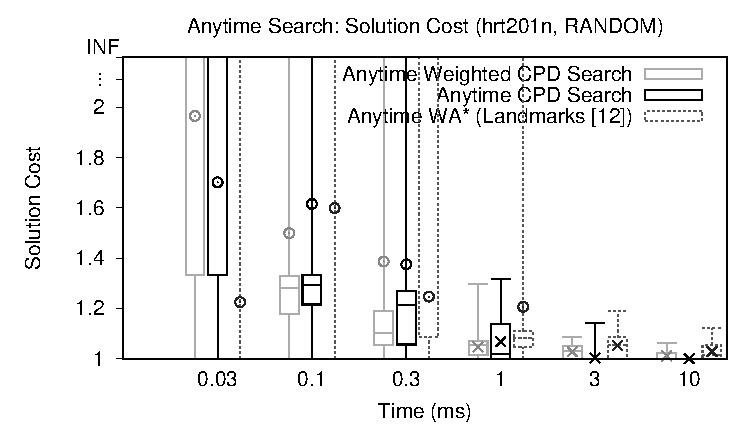
\includegraphics[width=1.0\textwidth]{src/images/anytime/anytime01}
        \label{fig:anytime01}
    \end{figure}
\end{frame}
